\section{Introduction to Multi-Robot Systems}

\begin{frame}
	\frametitle{Multi-Robot System (MRS)}
	
	\Large
	
	\begin{itemize}
		\item \textbf{a team of robots}
			
			\begin{itemize}
				\item homogeneous/heterogeneous
				
				\item sensors (laser, camera,...)
				
				\item actuators (wheels, legs,...)
			\end{itemize}			
		\item \textbf{a communication protocol}
			
			\begin{itemize}
				\item what information are shared
				
				\item how?
			\end{itemize}
		\item \textbf{assumptions}
			
			\begin{itemize}
				\item synchronized clock
				
				\item messages delivered in at most \emph{n} seconds
				
				\item ...
			\end{itemize}
	\end{itemize}
\end{frame}

\begin{frame}
	\frametitle{How do we can evaluate a MRS?}
	
	\Large
	
	\begin{itemize}
		\item Task dependent
		
		\begin{itemize}
			\normalsize
			
			\item object estimation accuracy (tracking system)
			
			\item time needed to built a map (SLAM)
		\end{itemize}
		
		\item Task independent
		
		\begin{itemize}
			\normalsize
			
			\item algorithm frame rate
			
			\item network usage and overhead
		\end{itemize}
	\end{itemize}
	
	\textbf{Different from simulated and real environments}	
	
	\begin{itemize}
		\normalsize
		
		\item Ground-truth acquisition\\
		
		\vspace{-0.2cm}
		
		\begin{tabbing}
			\hspace*{0.3cm}
			simulation $ \leadsto $ \textbf{easy} but \textbf{no} realistic results\\
			
			\hspace*{0.3cm}
			real $ \leadsto $ \textbf{difficult} but accurate results
		\end{tabbing}
	\end{itemize}
\end{frame}

\begin{frame}
	\frametitle{Guidelines for a good evaluation}
	
	\Large
	
	\begin{itemize}
		\item choose significant metrics
		
		\item standard simulators
		
		\vspace{-0.2cm}
		
		\begin{tabbing}
			\normalsize
			\hspace*{0.4cm}
			$ \leadsto $ Player/Stage (2D simulation) \\
			
			\normalsize
			\hspace*{0.4cm}
			$ \leadsto $ Gazebo (3D simulation)
		\end{tabbing}
		
		\item possible to compare with similar works in the literature
		
		\item hopefully used by the community as \textbf{benchmark}
	\end{itemize}
\end{frame}

\begin{frame}
	\frametitle{Multi-Object Detection and Tracking}
	\framesubtitle{A brief overview}
	
	\begin{columns}[t]
		\column{0.65\textwidth}
		\centering
		
		\only<1->
		{
			\vspace{0.2cm}
		}
		
		\only<1->
		{
			\begin{block}{Moving Object Detection}
				real-time extraction of moving objects from sensors
			\end{block}
		}
		
		\only<1>
		{
			\vspace{2.84cm}
		}
		
		\vspace{1.0cm}
		
		\only<2>
		{
			\begin{block}{Object Tracking\cite{Yilmaz06}}
				continuous observation of the objects over time to form persistent trajectories of the objects
			\end{block}
		}
		
		\column{0.3\textwidth}
		\centering
		
		\only<1->
		{
			\begin{tikzpicture}
				\node at (0,0) [draw=black,ultra thick,inner sep=0pt]  {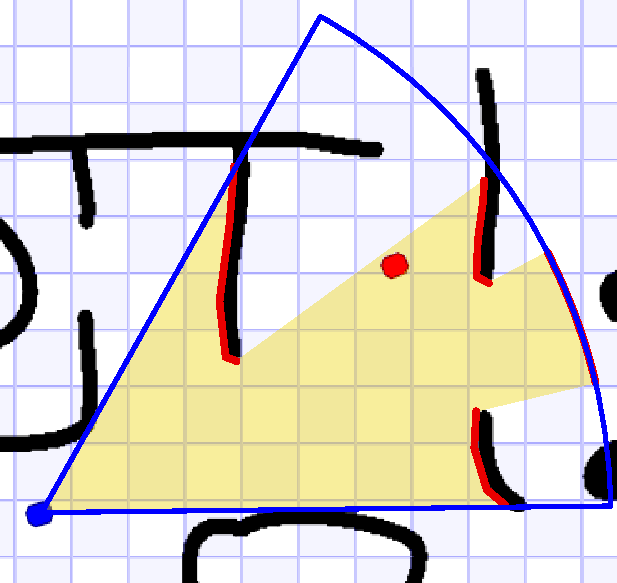
\includegraphics[scale=0.25]{Figures/Agent}};
			\end{tikzpicture}
		}
		
		\vspace{0.5cm}
		
		\only<2>
		{
			\begin{tikzpicture}
				\node at (0,0) [draw=black,ultra thick,inner sep=0pt] {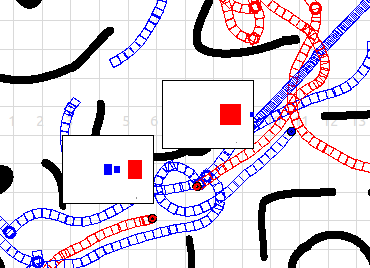
\includegraphics[scale=0.25]{Figures/Stage.png}};
			\end{tikzpicture}
		}
	\end{columns}
	
	\vspace{0.5cm}
	
	\begin{columns}
		\column{1.0\textwidth}
		
		\only<2>
		{
			\vspace{0.2cm}
		}
		
		\only<2->
		{
			\tiny 8. \emph{A. Yilmaz, O. Javed and M. Shah, ``Object tracking: A survey'' in Journal ACM Computing Surveys (CSUR), 2006}
		}
	\end{columns}
	
	\only<1>{\vspace{6cm}}
	\only<2>{\vspace{4cm}}
\end{frame}
